% !TEX TS-program = XeLaTeX
% use the following command:
% all document files must be coded in UTF-8
\documentclass[portuguese]{textolivre}
% build HTML with: make4ht -e build.lua -c textolivre.cfg -x -u article "fn-in,svg,pic-align"

\journalname{Texto Livre}
\thevolume{19}
%\thenumber{1} % old template
\theyear{2026}
\receiveddate{\DTMdisplaydate{2025}{7}{25}{-1}} % YYYY MM DD
\accepteddate{\DTMdisplaydate{2025}{10}{27}{-1}}
\publisheddate{\DTMdisplaydate{2026}{2}{12}{-1}}
\corrauthor{Thiago Costa da Silva}
\articledoi{10.1590/1983-3652.2026.60591}
%\articleid{NNNN} % if the article ID is not the last 5 numbers of its DOI, provide it using \articleid{} commmand 
% list of available sesscions in the journal: articles, dossier, reports, essays, reviews, interviews, editorial
\articlesessionname{articles}
\runningauthor{Silva, Silva e Giesel} 
%\editorname{Leonardo Araújo} % old template
\sectioneditorname{Daniervelin Pereira~\orcid{0000-0003-1861-3609}}
\layouteditorname{Saula Cecília~\orcid{0009-0006-3069-8480}}

\title{O domínio do corpo feminino: uma análise semiolinguística da Carta Aberta mediante as violências contra Klara Castanho na rede social Twitter/X}
\othertitle{The domination of the female body: a semiolinguistic analysis of the Open Letter regarding the violence against Klara Castanho on the social network Twitter/X}
% if there is a third language title, add here:
%\othertitle{Artikelvorlage zur Einreichung beim Texto Livre Journal}

\author[1]{Thiago Costa da Silva~\orcid{0000-0001-5884-2639}\thanks{Email: \href{mailto:thiago_cs@id.uff.br}{thiago\_cs@id.uff.br}}}
\author[1]{Patrick Neves de Paula da Silva~\orcid{0000-0002-6804-7812}\thanks{Email: \href{mailto:patricknps@id.uff.br}{patricknps@id.uff.br}}}
\author[2]{Cláudia Cristina Mendes Giesel~\orcid{0000-0001-6958-2377}\thanks{Email: \href{mailto:claudia.giesel@uva.br}{claudia.giesel@uva.br}}}
\affil[1]{Universidade Federal Fluminense, Niterói, RJ, Brasil.}
\affil[2]{Universidade Veiga de Almeida, Rio de Janeiro, RJ, Brasil.}

\addbibresource{article.bib}
% use biber instead of bibtex
% $ biber article

% used to create dummy text for the template file
\definecolor{dark-gray}{gray}{0.35} % color used to display dummy texts
\usepackage{lipsum}
\SetLipsumParListSurrounders{\colorlet{oldcolor}{.}\color{dark-gray}}{\color{oldcolor}}

% used here only to provide the XeLaTeX and BibTeX logos
\usepackage{hologo}

% if you use multirows in a table, include the multirow package
\usepackage{multirow}

% provides sidewaysfigure environment
\usepackage{rotating}

% CUSTOM EPIGRAPH - BEGIN 
%%% https://tex.stackexchange.com/questions/193178/specific-epigraph-style
\usepackage{epigraph}
\renewcommand\textflush{flushright}
\makeatletter
\newlength\epitextskip
\pretocmd{\@epitext}{\em}{}{}
\apptocmd{\@epitext}{\em}{}{}
\patchcmd{\epigraph}{\@epitext{#1}\\}{\@epitext{#1}\\[\epitextskip]}{}{}
\makeatother
\setlength\epigraphrule{0pt}
\setlength\epitextskip{0.5ex}
\setlength\epigraphwidth{.7\textwidth}
% CUSTOM EPIGRAPH - END

% to use IPA symbols in unicode add
%\usepackage{fontspec}
%\newfontfamily\ipafont{CMU Serif}
%\newcommand{\ipa}[1]{{\ipafont #1}}
% and in the text you may use the \ipa{...} command passing the symbols in unicode

% LANGUAGE - BEGIN
% ARABIC
% for languages that use special fonts, you must provide the typeface that will be used
% \setotherlanguage{arabic}
% \newfontfamily\arabicfont[Script=Arabic]{Amiri}
% \newfontfamily\arabicfontsf[Script=Arabic]{Amiri}
% \newfontfamily\arabicfonttt[Script=Arabic]{Amiri}
%
% in the article, to add arabic text use: \textlang{arabic}{ ... }
%
% RUSSIAN
% for russian text we also need to define fonts with support for Cyrillic script
% \usepackage{fontspec}
% \setotherlanguage{russian}
% \newfontfamily\cyrillicfont{Times New Roman}
% \newfontfamily\cyrillicfontsf{Times New Roman}[Script=Cyrillic]
% \newfontfamily\cyrillicfonttt{Times New Roman}[Script=Cyrillic]
%
% in the text use \begin{russian} ... \end{russian}
% LANGUAGE - END

% EMOJIS - BEGIN
% to use emoticons in your manuscript
% https://stackoverflow.com/questions/190145/how-to-insert-emoticons-in-latex/57076064
% using font Symbola, which has full support
% the font may be downloaded at:
% https://dn-works.com/ufas/
% add to preamble:
% \newfontfamily\Symbola{Symbola}
% in the text use:
% {\Symbola }
% EMOJIS - END

% LABEL REFERENCE TO DESCRIPTIVE LIST - BEGIN
% reference itens in a descriptive list using their labels instead of numbers
% insert the code below in the preambule:
%\makeatletter
%\let\orgdescriptionlabel\descriptionlabel
%\renewcommand*{\descriptionlabel}[1]{%
%  \let\orglabel\label
%  \let\label\@gobble
%  \phantomsection
%  \edef\@currentlabel{#1\unskip}%
%  \let\label\orglabel
%  \orgdescriptionlabel{#1}%
%}
%\makeatother
%
% in your document, use as illustraded here:
%\begin{description}
%  \item[first\label{itm1}] this is only an example;
%  % ...  add more items
%\end{description}
% LABEL REFERENCE TO DESCRIPTIVE LIST - END


% add line numbers for submission
%\usepackage{lineno}
%\linenumbers

\usepackage{xurl}

\begin{document}
\maketitle

\begin{polyabstract}
\begin{abstract}
O presente artigo, visando realizar uma análise semiolinguística, apresenta como pressuposto o fato de que a sociedade brasileira atual, seguindo uma longa tradição patriarcal e machista, realiza a perpetuação de um imaginário sociodiscursivo que condiciona as mulheres a uma posição histórico-social de menos prestígio que os homens, tanto na realidade quanto nas redes sociais. No dia vinte e cinco de junho de 2022, a atriz brasileira Klara Castanho, à época com vinte e dois anos, divulgou, em seu Twitter/X e Instagram, uma Carta Aberta na qual afirmava que havia sido vítima de estupro. Esta pesquisa tem por objetivo geral identificar os recursos linguístico-discursivos contidos na Carta Aberta postada por Klara Castanho e analisar os \textit{efeitos de sentido}. Para tanto, basear-nos-emos, principalmente, em \textcite{charaudeau2005, charaudeau2015, charaudeau2018, charaudeau2019} por abordar os conceitos de \textit{semiotização de mundo, imaginários sociodiscursivos, ethos e pathos} e em \textcite{hooks2019}, por trazer importantes contribuições sobre uma reflexão acerca do feminino. Em síntese, foi possível averiguarmos em que princípios o texto foi pautado e quais foram os seus possíveis \textit{efeitos pretendidos}. Verificamos que a criação de uma imagem de si, pautada na credibilidade e na identificação, é capaz de gerar um efeito patêmico no público-alvo.

\keywords{Teoria semiolinguística\sep Klara Castanho\sep Violência\sep Redes sociais\sep Feminino}
\end{abstract}

\begin{english}
\begin{abstract}
The present article, aiming to carry out a semiolinguistic analysis, has as its assumption the fact that current Brazilian society, following a long patriarchal and sexist tradition, carries out the perpetuation of a socio-discursive imaginary that conditions women to a historical-social position of less prestige than men, both in reality and on social media. On June 25, 2022, Brazilian actress Klara Castanho, then twenty-two years old, published an Open Letter on her Twitter/X and Instagram in which she stated that she had been a victim of rape. This research has the general objective of identifying the linguistic-discursive resources contained in the Open Letter posted by Klara Castanho and analyzing the \textit{effects of meaning}. To do so, we will base ourselves mainly on \textcite{charaudeau2005, charaudeau2015, charaudeau2018, charaudeau2019}, for addressing the concepts of \textit{semiotization of the world, socio-discursive imaginaries, ethos} and \textit{pathos}, and on \textcite{hooks2019}, for bringing important contributions on a reflection about the feminine. In short, it was possible to determine the principles on which the text was based and what its possible \textit{effects were predicted}. We found that creating an image of oneself, based on credibility and identification, is capable of generating a pathetic effect on the target audience.


\keywords{Semiolinguistic theory\sep Klara Castanho\sep Violence\sep Social media\sep Feminine}
\end{abstract}
\end{english}
% if there is another abstract, insert it here using the same scheme
\end{polyabstract}

\section{Introdução}\label{sec-intro}
A sociedade brasileira atual, seguindo uma longa tradição patriarcal e machista, realiza a perpetuação de um \textit{imaginário sociodiscursivo} que condiciona as mulheres a uma posição histórico-social de menos prestígio que os homens. Com o avanço dos movimentos feministas, faz-se presente, desde o século XX, no Brasil, a luta por equidade e por melhores condições para exercer uma cidadania plena, como a igualdade salarial, o respeito e a garantia para terem o controle sobre o próprio corpo. Contudo, contemporaneamente, as mulheres ainda sofrem com a dominação masculina sobre o seu destino, mesmo quando essas são acometidas por violência sexual.

No dia vinte e cinco de junho de 2022, a atriz brasileira Klara Castanho, à época com vinte e um anos, divulgou em seu perfil oficial do Instagram e do Twitter/X uma Carta Aberta na qual afirmava ter sido vítima de estupro. Apesar de a atriz ter declarado que nunca foi a sua intenção tornar esse fato público, isso se fez necessário pois supostamente uma profissional da área da saúde, logo após o procedimento do parto, que ocorreu em sigilo legal, teria comunicado o acontecimento a um jornalista\footnote{Em fevereiro de 2025, a justa causa da enfermeira acusada de expor os dados da atriz foi revertida. A justiça entendeu que não há provas de que a enfermeira ou seu marido vazaram os dados para a imprensa.
 \newline MORAIS, M. Enfermeira acusada de vazar parto de Klara Castanho tem vitória na Justiça. \textit{Site Correio Braziliense} 07 fev. 2025, 09h29. Disponível em: \url{https://www.correiobraziliense.com.br/colunistas/mariana-morais/2025/02/7054917-enfermeira-acusada-de-vazar-parto-de-klara-castanho-tem-vitoria-na-justica.html}. Acesso em: 03 jun. 2025.}. Em pouco tempo, a informação tornou-se conhecida, o que levou a atriz a um julgamento moral baseado no senso comum como, por exemplo, o ``atrevimento'' de uma mulher ao entregar um bebê para adoção.

Tendo em vista as violências cometidas contra Klara Castanho, tanto física quanto psicológicas, o presente trabalho propõe-se a investigar, mediante a análise semiolinguística do discurso, na Carta Aberta publicada em sua rede social, as seguintes questões:

\begin{enumerate}
    \item qual foi a estratégia linguístico-discursiva que a atriz brasileira utilizou para captar a atenção do público brasileiro e produzir os efeitos de sentido pretendidos?
    \item como a carta menciona os argumentos levantados pelo médico e pela enfermeira e em que medida esses argumentos perpetuam o domínio do corpo feminino?
    \item como a carta se refere aos boatos e o modo como eles contribuem com a violência contra a mulher bem como a reprodução de papéis de gênero?
\end{enumerate}

Frente aos questionamentos propostos, este artigo assume como objetivo geral identificar os recursos linguístico-discursivos contidos na Carta Aberta postada por Klara Castanho e analisar os efeitos de sentido pretendidos pela atriz. Como objetivos específicos, pretende-se verificar como os efeitos de \textit{pathos} (convencimento pela emoção) podem ter sido utilizados para sensibilizar os leitores; explorar os argumentos dos profissionais de saúde relatados na carta que tentaram persuadir a atriz a não entregar a criança para a adoção; verificar o \textit{ethos} (uma imagem de si) de credibilidade e de identificação e certificar, por meio do \textit{corpus}, que a propagação de informações incorretas, na internet, pode ocasionar prejuízos emocionais aos sujeitos que se tornam alvo de sofrimento.

Diante dos questionamentos aqui formulados, pretende-se, neste artigo, por intermédio da análise semiolinguística do discurso, averiguar as seguintes hipóteses:

\begin{enumerate}
    \item a atriz Klara Castanho utilizou um forte apelo às emoções para que os usuários do Twitter/X e Instagram fossem captados pelo seu discurso e para que as especulações e os julgamentos sobre a sua atitude fossem cessados;
    \item foram utilizados argumentos balizados no apelo ao papel social atribuído à mulher, à questão biológica e à chantagem emocional;
    \item os boatos e ilações colocaram a atriz em posição de vulnerabilidade e originaram ataques em relação à sua decisão sobre o destino do recém-nascido.
\end{enumerate}

Aliado a isso, este trabalho apresenta como justificativa social e acadêmica o fato de que o \textit{corpus} reforça a relevância sobre a temática da violência e domínio sobre o corpo feminino como um tema sensível e de interesse para o campo da Semiolinguística, como a estratégia de \textit{patemização} (mobilização de recursos intralinguísticos e extralinguísticos que visam a captar o interlocutor por meio da emoção) e \textit{encenação discursiva}\footnote{Para \textcite{charaudeau2019}, a encenação discursiva é uma atividade de teatralização presente em todo ato de linguagem, tendo em vista que cada interação humana dar-se-ia por meio de uma \textit{encenação} entre, no mínimo, dois parceiros sociais.}. Ao serem encontrados comentários de homens e mulheres em redes sociais acerca do comportamento assumido por Klara Castanho, pode-se perceber que há uma pressão sobre o que é esperado de uma mulher-mãe. No Brasil, apesar do avanço dos movimentos feministas, a antiga tradição patriarcal e machista moldou o pensamento segundo o qual existiriam ``coisas de homem'' e ``coisas de mulher''. O cuidado com os filhos e do lar foi atribuído historicamente às mulheres, enquanto aos homens foi conferida a responsabilidade financeira. Mediante isso, muitos julgamentos foram realizados contra a atriz (\Cref{fig-1}).

%--- codigo da figura 1 ---%
\begin{figure}[h!]
\centering
\begin{minipage}{.90\textwidth}
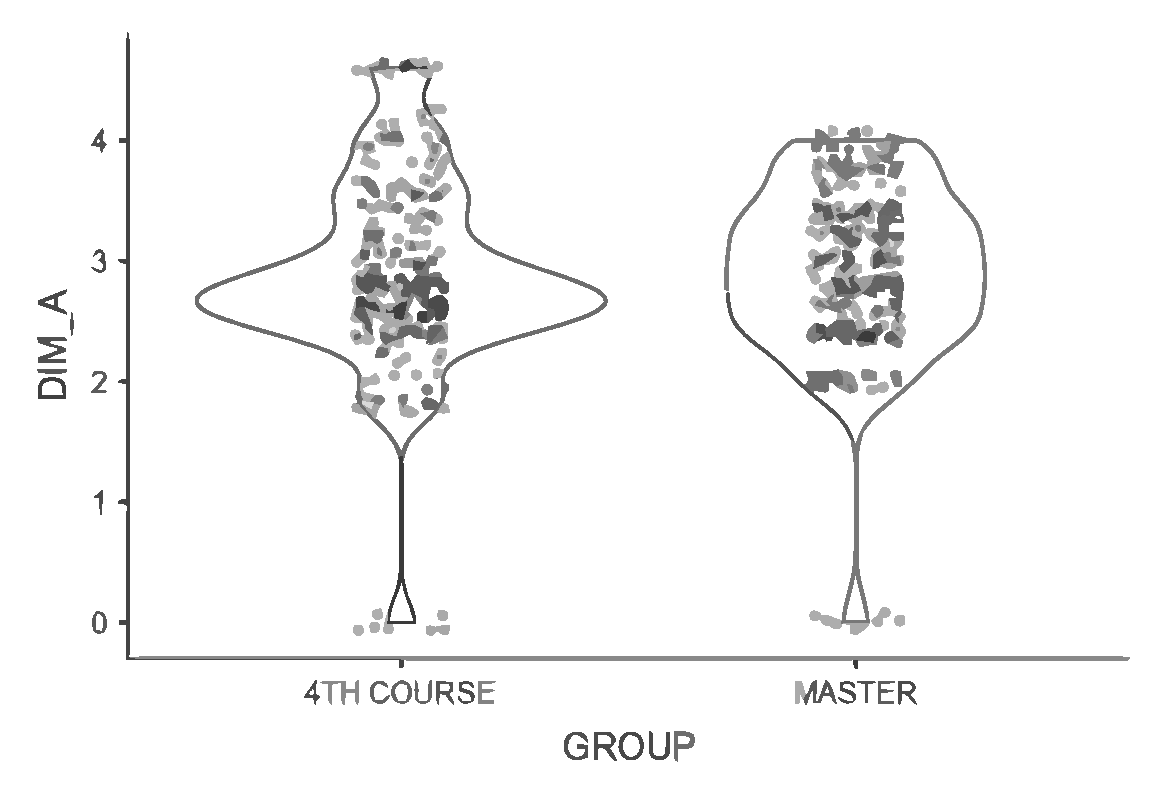
\includegraphics[width=\textwidth]{Imagens/fig1.png}
\caption{Compilado de alguns \textit{tweets} extraídos da rede social Twitter/X em relação ao caso Klara Castanho, depois da publicação da Carta Aberta.}
\label{fig-1}
\source{Disponível em: \url{https://x.com/KlaraCastanho/status/1534353229886234624}, \url{https://x.com/KlaraCastanho/status/1532106193778376704} e \url{https://x.com/BbbPsicologa/status/1541240488040321024}. Acesso em: 05 fev. 2026.}
\end{minipage}
\end{figure}

Independentemente de sabermos se os comentários, em tom de acusação, sarcasmo, deboche e insensibilidade, foram produzidos por homens ou mulheres, pela não confiabilidade da autenticidade do nome de usuário e da fotografia de perfil, é perceptível, por meio dos atos de linguagem selecionados anteriormente, a tentativa de dominação do corpo feminino. 

O presente artigo apresenta caráter qualitativo. Em relação a isso, utilizaremos o método exploratório, considerando a propensão em criar-se uma familiaridade com o objeto a ser analisado, descrito e classificado pelo pesquisador, além de um levantamento bibliográfico, que proporcionará o contato com a Carta Aberta e com os \textit{efeitos de sentido} possíveis.

Em decorrência da proposta de análise e de investigação de nosso trabalho, utilizaremos o método e a técnica de pesquisa de estudo de caso, tendo em vista que pretendemos compreender como os sujeitos comunicante e enunciador -- a atriz Klara Castanho -- construíram o texto para convencer os sujeitos interpretante e destinatário -- os leitores brasileiros -- de que os seus comportamentos foram os melhores possíveis, tendo em vista prezar pelo bem-estar da criança e por preservar a sua imagem.

Para isso, utilizaremos a Semiolinguística como aporte teórico-metodológico para a análise do \textit{corpus}, pois compreendemos que essa teoria apresenta as ferramentas necessárias para conduzir a proposta do estudo. A investigação em desenvolvimento neste artigo concentra-se, principalmente, nas obras do linguista francês Patrick Charaudeau \citeyear{charaudeau2005, charaudeau2015, charaudeau2018, charaudeau2019}, por abordarem os conceitos de \textit{Semiotização de mundo, imaginários sociodiscursivos, ethos} e \textit{pathos} e em \textcite{hooks2019}\footnote{Este nome é escrito em letra minúscula por razões políticas, ideológicas e de resistência.}, por trazer importantes contribuições sobre o feminino.

\section{Carta Aberta: a dor e o parecer feminino de Klara Castanho}
Nesse sentido, realizaremos uma breve contextualização do caso Klara Castanho. Houve três episódios que foram decisivos para que o nome da atriz fosse envolvido em ilações quanto à sua maternidade. O primeiro foi protagonizado pelo jornalista Matheus Baldi\footnote{F5. Klara Castanho: jornalista que expôs o caso é demitido. \textit{Folha de São Paulo}, 16. jul. 2022, 18h34. Disponível em: \url{https://f5.folha.uol.com.br/celebridades/2022/07/klara-castanho-jornalista-que-expos-o-caso-e-demitido.shtml}. Acesso em: 15 nov. 2025.
}, no dia 24 de maio de 2022, que, por meio de uma postagem em seu Instagram, afirmou que a atriz havia dado à luz a uma criança há cerca de quinze dias. Por pedidos da própria jovem, a informação foi deletada, porém seu nome já estava circulando nas redes sociais.

O segundo foi protagonizado pelo jornalista brasileiro Leo Dias\footnote{Leonardo Antônio Lima Dias.}, em uma entrevista concedida ao programa ``The Noite'', com Danilo Gentili, exibida no SBT, no dia 16 de junho de 2022, que afirmou que uma atriz recentemente realizara um ato infeliz, que poderia causar uma repercussão muito negativa para a sua vida e carreira, e assegurando que ``o karma vai ser grande''\footnote{ Fala transcrita de Leo Dias durante a entrevista.
	THE NOITE COM DANILO GENTILI. Entrevista com Leo Dias | The Noite (16/06/22). \textit{YouTube}, 17 jun. 2025. Disponível em: \url{https://www.youtube.com/watch?v=8L-aZnhHO7M}. Acesso em: 15 nov. 2025.}. Além disso, segundo o colunista, essa mulher estava enganando todo o povo brasileiro e sua atitude envolvia o impacto em vidas alheias; com isso, a imagem de ``santinha'' criada por essa atriz seria desfeita.

    O terceiro episódio foi protagonizado pela \textit{youtuber} e apresentadora brasileira Antônia Fontenelle \cite{splash2022dias_fontenelle}, em uma \textit{live}, no dia 23 de junho de 2022. Sem citar o nome de Klara Castanho, Fontenelle, em tom de acusação, afirmou, ``com base em provas'', que uma atriz da Rede Globo, de vinte e um anos, teria engravidado, ocultado esse fato do público e entregado o recém-nascido à adoção. Além disso, teria pedido para que a direção do hospital em que o procedimento ocorreu apagasse todos os registros que provassem sua passagem pela instituição e teria solicitado que levassem o seu filho para longe de si, cometendo o crime de ``abandono de incapaz''. Em sequência a esse acontecimento, a jovem decidiu manifestar-se sobre o assunto por meio da Carta Aberta em seus perfis oficiais.

\section{Teoria Semiolinguística}
Patrick Charaudeau, ao desenvolver sua Teoria Semiolinguística de Análise do Discurso, embasou-se em alguns conhecimentos acadêmicos modernos, como o dialogismo de Bakhtin, a enunciação de Benveniste e a filosofia da linguagem, de Austin, Searle e Grice. \textcite{charaudeau2018}, em seus estudos linguísticos para a investigação dos \textit{efeitos de sentido pretendidos} por sujeitos produtores de um \textit{ato de linguagem}, também sofreu influência teórica de Aristóteles, em sua Retórica Clássica, ao retomar os estudos do \textit{ethos} e do \textit{pathos} em sua Teoria Semiolinguística para a investigação da \textit{captação} do público/auditório.

O \textit{Ethos} consiste na criação da imagem de si que os sujeitos interlocutores realizam durante a interação. Para \textcite{charaudeau2018}, não existe um \textit{ato de linguagem} sequer que não passe por esse processo de construção de uma máscara que utilizamos para interagirmos com o outro.

\begin{quote}
    Quer queiramos ou não, calculemos ou neguemos, a partir do momento em que falamos, aparece (transparece) uma imagem daquilo que somos por meio daquilo que dizemos. Não se trata tanto de nosso posicionamento ideológico, do conteúdo de nosso pensamento, de nossa opinião, quanto daquilo que sobressai da relação que mantemos conosco e que oferecemos à percepção dos outros \cite[p. 86]{charaudeau2018}.
\end{quote}

A construção de um \textit{ethos}, dessa forma, ocorre de forma não completamente dependente da vontade dos sujeitos em interação e é inerente aos atos linguageiros. Apesar disso, esse conceito é passível de manipulação, tendo em vista que essa construção imagética pode ser criada e recriada em diferentes \textit{atos de linguagem}. Quando um político sobe ao palco para fazer uma declaração oficial de seu governo, as suas palavras, o ritmo, a entonação, sua vestimenta e a maneira de se dirigir aos outros fazem parte da criação de seu \textit{ethos} político, visando conquistar a confiança e a credibilidade e preservar sua legitimidade perante a opinião pública. A construção dessa imagem pode dar-se por meio do apelo à emoção ou à razão.

Para \textcite{amossy2016}, a apresentação de si é tributária dos papéis sociais e do contexto situacional e, tendo em vista sua inerência à interação, ela supera largamente a intencionalidade do sujeito que fala e age. Além disso, ``o que'' e ``como'' nós falamos deve respeitar os \textit{ritos de interação}; para \textcite{goffman2011}, isso se refere aos comportamentos que são esperados para um ato de linguagem, tendo em vista cumprir com as expectativas criadas em torno dos sujeitos interagentes e do gênero discursivo. Klara Castanho, antes de redigir o seu texto, além de ter que escolher as características do material linguageiro, o que impactaria na natureza de sua escrita, deverá cumprir com as expectativas de sua forma e de seu conteúdo. Ao escrever a Carta Aberta, qual é a imagem que a atriz quis criar de si?

O outro conceito retomado por \textcite{charaudeau2018} é o de \textit{Pathos}. Este se refere ao apelo à emoção que o sujeito que se comunica realiza para captar a atenção de seu público; essa sedução ou persuasão pode dar-se por meio de suas palavras e de seus comportamentos. De acordo com o linguista francês, um discurso pode produzir um efeito emocional (também chamado de patêmico) no auditório conforme são combinados três fatores: (i) a natureza do universo de \textit{crença}\footnote{Os conceitos \textit{saber de crença} e \textit{saber de conhecimento} serão abordados a seguir.} ao qual o discurso faz referência (vida/morte, amor, catástrofe, crime, paixão, estupro); (ii) a encenação discursiva que poderá, por si mesma, parecer dramática, trágica, espetacular ou neutra e (iii) o posicionamento assumido pelo interlocutor (público-alvo) em relação aos universos de crença convocados e o estado de espírito atual da plateia.

Tendo isso em vista, podemos afirmar que há temáticas que são mais ou menos patêmicas; o estupro, por exemplo, na cultura brasileira, é um crime que influencia as emoções. Contudo, não basta apenas falar/escrever sobre um assunto: o modo com que a atriz abordou esse tópico é tão importante quanto o tema. Geralmente uma mulher que sofreu violência sexual não vai prestar depoimento sorrindo ou em tom de deboche; as suas palavras e seu comportamento têm que compor uma unidade e ir ao encontro do \textit{rito de interação} esperado para o \textit{ato de linguagem}. Além disso, o leitor dessa enunciação deve possuir um julgamento similar ao do sujeito que produz a mensagem do que seja o estupro. Se por acaso a atriz Klara Castanho estivesse escrevendo sua Carta Aberta tendo em vista afetar emocionalmente um auditório composto por indivíduos que culpabilizam a mulher pelo crime, o efeito patêmico provavelmente não teria sido concretizado.

\section{Processo de semiotização de mundo}
Outro conceito que será utilizado para realizarmos a análise do \textit{corpus} é o de \textit{semiotização de mundo}, desenvolvido por Charaudeau. Segundo este linguista, para que possamos nos comunicar com o outro, é necessário realizarmos um duplo processo. O primeiro é chamado de \textit{processo de transformação}, que consiste em converter um ``mundo a significar'' em um ``mundo significado'', ou seja, o sujeito falante/escritor seleciona as palavras da língua e as combina para \textit{significar o mundo} e conseguir construir uma mensagem com sentido para seu interlocutor. O segundo procedimento é conhecido como \textit{processo de transação}, em que o sujeito que produziu o ``mundo significado'' vai utilizar este texto como um objeto de troca com o outro interagente. Reproduziremos a seguir o quadro realizado pelo autor para ilustrar essa dinâmica comunicacional (\Cref{fig-2}).

%--- codigo da figura quadro 1 ---%
\begin{figure}[h!]
\centering
\begin{minipage}{.90\textwidth}
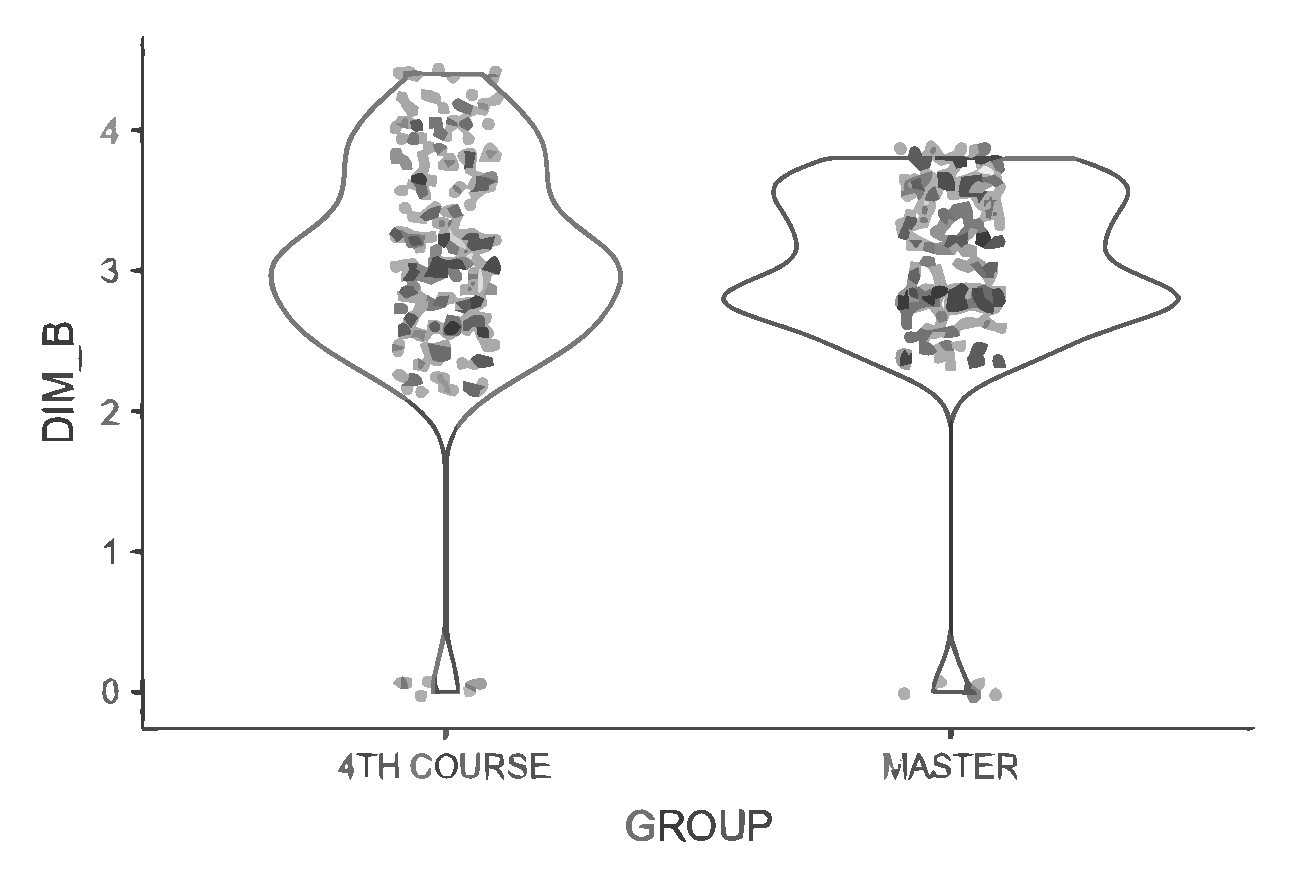
\includegraphics[width=\textwidth]{Imagens/fig2.png}
\caption{O processo de transação e o processo de transformação.}
\label{fig-2}
\source{Adaptado de \textcite[p. 14]{charaudeau2005}.}
\end{minipage}
\end{figure}

O \textit{processo de transformação} é composto por quatro categorias: \textit{identificação, qualificação, ação e causação}. A \textit{identificação} consiste no emprego de substantivos e de pronomes utilizados para fazer referência a seres que podem ser encontrados em um \textit{ato de linguagem}. Esses, tendo isso em vista, são convertidos em ``identidades nominais''. A \textit{qualificação}, que consiste na atribuição de características positivas ou negativas, de forma explícita ou implícita, aos seres de um enunciado, pode ser identificada por meio de adjetivos, orações adjetivas, orações reduzidas, substantivos ou quaisquer outras categorias gramaticais que desempenham esse papel \cite{charaudeau2015}. Estes seres, por sua vez, são transformados em ``identidades descritivas''. A \textit{ação} é o resultado de um ato sofrido ou praticado por um sujeito em um enunciado, o que lhe atribui a qualidade de ``identidade narrativa''. Por fim, a \textit{causação} é classificada como a motivação, humana ou não humana, pela qual os seres são inscritos em uma cadeia de causalidade. Essa última operação introduz os sujeitos interlocutores em ``relações de causalidade'', em uma lógica de causa e efeito. Podemos identificar essa classe por meio das conjunções utilizadas, por exemplo.

Quanto ao \textit{processo de transação}, \textcite{charaudeau2005} classifica-o em quatro categorias: o \textit{princípio de alteridade, o princípio de pertinência, o princípio de influência} e o \textit{princípio de regulação}. O primeiro consiste no fenômeno de interlocução entre, no mínimo, dois sujeitos, seja em um texto dialogal ou monologal, em que temos um duplo processo de identificação de semelhanças e diferenças em relação ao outro. A similaridade deve-se à primordialidade na encenação de reconhecermos, no nosso interlocutor, um \textit{universo de referências} (saberes afins); a dessemelhança deve-se não só pelo fato de os sujeitos assumirem papéis diferentes no \textit{ato de linguagem} (falante/escritor e interlocutor), mas também à constatação de diferenças em relação à \textit{identidade} do outro, devido a fatores psicossociais, culturais e de trajetória de vida que nos diferenciam. É a partir desses traços distintivos, portanto, que conseguimos realizar a nossa construção identitária, pois entendemos que nós somos aquilo que o outro não é.

O \textit{princípio de pertinência} consiste no fato de os sujeitos interagentes possuírem conhecimentos compartilháveis entre si, durante a encenação. Para que, no mínimo, dois cidadãos consigam sustentar uma comunicação, é necessário que eles tenham em comum um universo de referências, não só sobre o outro interlocutor, mas também sobre o conteúdo. Para que um ``mundo significado'' seja aceito pelo outro sujeito, é preciso que esses saberes evocados estejam apropriados ao contexto e à finalidade comunicacional.

O \textit{princípio de influência} diz respeito ao processo que o sujeito produtor da mensagem desempenha para levar o seu interlocutor a uma ação, seja para guiar seus pensamentos, seja para manipular seus sentimentos, tendo em vista um proveito próprio. Apesar de muitas vezes os \textit{atos de linguagem} parecerem despretensiosos, toda comunicação humana visa influenciar o outro, o que faz com que devamos estar atentos a essa categoria, pois possivelmente ela carrega importantes pistas ideológicas do enunciador.

Por último, o \textit{princípio de regulação} refere-se precisamente à necessidade de haver um reconhecimento mínimo de saberes afins entre os interagentes em uma interlocução. Caso isso não aconteça, a interação pode não ocorrer de maneira orgânica, devido à falta de temas sobre os quais interagir ou a demais rupturas ao \textit{ato de linguagem} relacionadas aos demais aspectos contratuais. Esse princípio é de grande importância para que a comunicação ocorra, sendo que essa \textit{regulação} pode ser realizada de modo consciente ou não.

\section{Dialogismo}
Outro conceito caro a este artigo é o de dialogismo bakhtiniano. Para \textcite{brait1994}, Bakhtin afirma que tudo o que é dito por qualquer sujeito, tudo o que é expresso por um falante, não pertence só a ele. ``Em todo discurso são percebidas vozes, às vezes infinitamente distantes, anônimas, quase impessoais, quase imperceptíveis, assim como as vozes próximas que ecoam simultaneamente no momento da fala'' \cite[p. 15]{brait1994}. Tendo isso em vista, podemos afirmar que em todo enunciado produzido pelo homem, em todo posicionamento tomado sobre algum tema, somos atravessados por outras vozes, outros textos já elaborados por outras pessoas anteriormente. Não há, de fato, a confecção de uma mensagem nova, original, mas algo que é produto de nosso processamento mental em relação a ideias já existentes e lançadas nas interações humanas.

Para \textcite[p. 316]{bakhtin2000}, ``O enunciado está repleto dos ecos e lembranças de outros enunciados, aos quais está vinculado no interior de uma esfera comum da comunicação verbal. O enunciado deve ser considerado acima de tudo como uma resposta a enunciados anteriores [...]''. Quando tomamos como exemplo o fato de que o médico, mediante a narração e o \textit{dialogismo interdiscursivo} presente na Carta Aberta, tentou persuadir a atriz brasileira Klara Castanho a ficar com a criança, independentemente de ela ter sido concebida por uma violência sexual, utilizando argumentos biológicos e sociais (``[...] esse profissional me obrigou a ouvir o coração da criança, disse que 50\% do DNA eram meus e que eu seria obrigada a amá-lo''), podemos concluir que esse profissional, durante sua formação como cidadão, foi atravessado por discursos que condenam uma mulher por não desempenhar o papel social de mãe, apesar das circunstâncias.

\section{Das representações sociais aos imaginários sociodiscursivos}
Aliado ao conceito de \textit{dialogismo}, podemos afirmar que é por meio de \textit{representações sociais} que criamos nossa concepção sobre objetos do mundo. Para \textcite{moscovici2007fenomeno}, as nossas concepções sobre o mundo e a nossa resposta a estímulos estão condicionadas socialmente a uma mesma criação de imagens que os cidadãos de um mesmo grupo social compartilham.

\begin{quote}
Nenhuma mente está livre dos efeitos de condicionamento anteriores que lhe são impostos por suas representações, linguagem ou cultura. Nós pensamos através de uma linguagem; nós organizamos nossos pensamentos, de acordo com um sistema que está condicionado, tanto por nossas representações, como por nossa cultura. Nós vemos apenas o que as convenções subjacentes nos permitem ver e nós permanecemos inconscientes dessas convenções \cite[p. 35]{moscovici2007fenomeno}.
\end{quote}

Para compreendermos a constituição das \textit{representações sociais} e como o processamento mental sobre o mundo e sobre a realidade dá origem aos \textit{imaginários}, temos que compreender o \textit{saber de crença} e o \textit{saber de conhecimento} \cite{charaudeau2022, charaudeau2025}. No interior das sociedades humanas, há a presença desses dois tipos de saberes, que apresentam uma dinâmica e um impacto social diferentes.

O \textit{saber de crença} refere-se ao julgamento dos fenômenos do mundo por meio de valores que atribuímos, tendo em vista explicar a realidade de um modo dissociado das percepções humanas (``a Terra é esférica''). Esses valores são constituídos por um juízo não relativo ao \textit{conhecimento de mundo} (``a questão não é saber se é bom ou ruim que a Terra seja esférica''), mas sim aos seres que fazem parte de uma comunidade social, de seus pensamentos e de seus comportamentos \cite{charaudeau2018}.

\begin{quote}
    Os saberes de crenças são procedentes de um movimento de avaliação, findo o qual o sujeito determina seu julgamento a respeito dos fatos. [...] Deve-se, portanto, admitir a existência de vários julgamentos possíveis. O sujeito que fala faz sua escolha segundo uma lógica do necessário e do verossímil, na qual pode intervir tanto a razão quanto a emoção. E já que existem vários julgamentos sobre o mundo, eles são objeto de confrontação ou de divisão. Todo juízo de crenças está fundado sobre uma partilha, pois se pode dizer que ele tem também uma função identitária (o que não acontece necessariamente com o saber de conhecimento). \cite[p. 198]{charaudeau2018}.
\end{quote}

Dessa forma, os \textit{saberes de crença}, por não serem baseados em fundamentos científicos, não apresentam um consenso em meio à sociedade em que estão difundidos. Esses julgamentos sobre o real podem ser concebidos por parte desse grupo social como sendo verdadeiros ou permitidos e, por outra, como falsos e ilegítimos, dividindo os seres sociais quanto a temáticas polêmicas, como política, religião, futebol e aborto \cite{charaudeau2022}. Referindo-se ao \textit{corpus} deste trabalho, que aborda a discriminação sofrida pela atriz por entregar o seu bebê recém-nascido à adoção, podemos encontrar justificativas na religião e no senso comum para atacar o comportamento de Klara Castanho, porém os argumentos sustentados pelos profissionais de saúde, ainda assim, não apresentariam um embasamento teórico.

Os \textit{saberes de conhecimento}, contudo, para \textcite{charaudeau2018}, apresentam fundamentação em uma base teórica sólida (como \textcite{castoriadis2000}) e visam a encontrar uma verdade quanto aos fenômenos do mundo.

\begin{quote}
    Esses saberes dizem respeito aos fatos do mundo e à explicação que se pode dar sobre o porquê ou o como desses fenômenos. Eles participam, portanto, de uma \textit{razão científica} que constrói uma representação da realidade que vale pelo conhecimento do próprio mundo \cite[p. 197, grifo do autor]{charaudeau2018}.
\end{quote}

Conforme os saberes de conhecimento e de crença, segundo \textcite{charaudeau2018}, agem na \textit{representação sociodiscursiva} do mundo significado pela linguagem em um ato linguageiro, trataremos de \textit{imaginários}. Levando em conta que estes estão presentes em enunciados realizados em diferentes materialidades semiológicas (escrita, fala, gesto, imagem), porém com similaridades semânticas, falaremos de \textit{imaginários discursivos}. Por último, pelo fato de essas imagens compartilhadas pela linguagem circularem em meio a grupos sociais, que constituem normas de referência, chamá-las-emos de \textit{imaginários sociodiscursivos} \cite{charaudeau2018}.

De acordo com \textcite[p. 205]{charaudeau2018}: ``[...] todo imaginário é um \textit{imaginário de verdade} que essencializa a percepção do mundo em um saber (provisoriamente) absoluto. O imaginário resulta de uma dupla interação: do homem com o mundo, do homem com o homem'' (grifo do autor). Esses saberes que circulam nos grupos sociais são materializados por meio de discursos que os legitimam. Para \textcite{charaudeau2018}, alguns desses discursos são veiculados por meio de textos escritos (ou orais), de modo mais ou menos estáveis, e transmitidos de geração em geração, como as teorias científicas e as doutrinas religiosas; já outros, são permeados na sociedade por meio de configurações mais mutáveis, como os provérbios e os ditados, mesmo que seu sentido seja semanticamente preservado. 

\section{Gênero discursivo ``Carta Aberta''}
Mediante a volatilidade inerente a alguns textos, faz-se de grande importância o conhecimento acerca das características do gênero discursivo que será alvo de análise neste artigo. A Carta Aberta, para \textcite[p. 20]{nunes2018}:

\begin{quote}
[...] é um gênero por meio do qual o escritor/remetente dirige-se ao seu leitor/destinatário publicamente para manifestar sua opinião sobre um fato, geralmente um problema social, a fim de fazer uma solicitação, uma reivindicação, um apelo ou um pedido. Tanto o remetente quanto o destinatário podem também consistir em um grupo de pessoas, em uma entidade, enfim, em uma coletividade.
\end{quote}

Acredita-se que a escolha de Klara Castanho em utilizar o gênero ``Carta Aberta'' cumpriu uma função informativa assertiva, pois a atriz, legitimamente, pôde realizar sua declaração sobre a origem de sua gravidez e, com isso, retirar o peso que as avaliações negativas exerciam sobre si. Pelo fato de esse gênero discursivo possuir uma finalidade formal, diferentemente de uma simples postagem em um \textit{feed}, um \textit{story} ou um \textit{reels}, possibilidades disponíveis na plataforma digital Instagram, ocorre, assim, uma quebra de expectativa em relação ao que se é esperado na rede social. Com isso, concomitantemente com o conteúdo sensível da mensagem propagada, foi possível que a mesma se tornasse amplamente difundida e comentada pelos leitores, cumprindo com a possível intenção da jovem.

\section{Feminino}
De acordo com \textcite{gomes2015}, a abordagem de gênero é um indicativo de que todas as práticas sociais, independentemente da esfera da vida do indivíduo, não são condicionadas biologicamente, mas sim permeadas por relações de gênero, as quais definem o que é ``ser homem'' e o que é ``ser mulher'', engendrando assim seus papéis de gênero por meio de relações de poder. Ainda para as autoras, é por meio dessa força hegemônica que ocorre não só a dominação, mas também a domesticação das mulheres.

\begin{quote}
    As relações saber-poder produzem a sexualidade (hétero), o sexo e o corpo (masculinos e femininos), o gênero (os papéis sociais do homem e da mulher). Tais construções são permeadas pelo biopoder (relações de poder exercidas através da gestão da vida, especialmente através da produção da sexualidade) e pelo poder patriarcal \cite[p. 209]{gomes2015}.
\end{quote}

Tendo isso em vista, as mulheres, desde muito pequenas, são socialmente condicionadas a pensarem e agirem de acordo com que o poder hegemônico as impõe. O fato de as meninas serem incentivadas a serem mais retraídas do que os meninos, tanto física (não se sentarem com as pernas abertas, por exemplo) quanto comportamentalmente (serem recatadas), cria sobre o imaginário do feminino uma imagem de fragilidade e de docilidade. Aliado a isso, por consequência de nossa sociedade ser regida pelo sistema patriarcal\footnote{``A cultura patriarcal exige a passividade feminina em todos os espaços: familiar, político, de trabalho -- ou seja, esses são espaços em que a autonomia da mulher é desrespeitada e em que há desqualificação do modo como ela exerce a sua sexualidade'' \cite[p. 78]{souza2019}.}, às mulheres foram atribuídas tarefas que giram em torno do âmbito domiciliar, em que o cuidado e o zelo fazem-se presentes. Ao não respeitar a essa expectativa social, o sexo feminino pode ser julgado como incompleto e sem realização pessoal.

Quando tocamos no ponto sensível de que a atriz Klara Castanho foi sexualmente violentada, temos que ter clara a distinção entre a imagem de \textit{vítima} e a de \textit{sofrimento}. ``[...] o sofrimento é o oposto da vitimização; é a experiência existencial da violência e injustiça à luz de valores que foram, evidentemente, derrotados e postos de lado ou rejeitados, mas também de valores que estão visceralmente vivos e que são visceralmente reconfortantes'' \cite[p. 141]{santos2019}. A importância de realizar-se essa diferenciação reside no fato de que, socialmente, o \textit{status} de ``vítima'' pode ser passível de relativização, enquanto o uso da palavra ``sofrimento'' remete a uma dor física ou psíquica que é universal ao ser humano.

Levando em conta o sofrimento causado à Klara Castanho, podemos aludir ao conceito de \textit{sofrimento injusto}, levantado por \textcite{santos2019}. Este martírio, segundo o autor, mesmo quando a mulher nada pode fazer para impedi-lo, é proveniente da ação do neoliberalismo para conseguir separar a ocorrência do sofrimento do sentimento de injustiça atrelado a ele. ``Tal separação visa criar indiferença perante o sofrimento de outrem e resignação perante o sofrimento próprio. Essa indiferença e essa resignação são os componentes básicos do novo fatalismo que paira atualmente sobre as sociedades capitalistas, colonialistas e patriarcais'' \cite[p. 144]{santos2019}. Com isso, mesmo quando a atriz realiza uma declaração pública sobre a sua dor, há pessoas que a acusam e que duvidam de que ela tenha falado a verdade ou que tenha tomado a melhor decisão.

Para a pesquisadora \textcite{hooks2019}, o movimento feminista contemporâneo possui como um de seus principais pilares a necessidade de se acabar com a violência dos homens contra as mulheres. Apesar de haver anos de lutas e conquistas, esse mal ainda se faz presente no século XXI. ``As ativistas feministas assumem frequentemente que esta violência é diferente de outras formas de violência nesta sociedade, pois está ligada especificamente às políticas do sexismo e da supremacia masculina: o direito dos homens de dominarem as mulheres'' \cite[p. 92]{hooks2019}. Tendo isso em vista, é possível de ser percebida, em muitos homens brasileiros, uma postura de se achar socialmente superior à mulher, em que comportamentos como o assédio e as violências moral, simbólica e até física podem ser concretizados. Em casos mais extremos, tem-se a ocorrência do estupro e, com isso,

\begin{quote}
    [...] o ato sexual como uma relação de dominação. De modo geral, possuir sexualmente [...] é dominar no sentido de submeter a seu poder, mas significa também enganar, abusar ou, como nós dizemos, ``possuir'' [...]. As manifestações (legítimas ou ilegítimas) da virilidade se situam na lógica da proeza, da exploração, do que traz honra \cite[p. 29]{bourdieu2012}.
\end{quote}

A violência sexual configura-se como a forma mais extrema de dominação masculina sobre o corpo feminino. Por outro lado, mesmo com o ato de subjugar e trazer sofrimentos à mulher, infelizmente, ainda se encontram justificativas em relação ao comportamento do público-alvo do abuso, como o comprimento da roupa, o fato de ``não se dar ao respeito'' e a ingestão de bebidas alcoólicas, atribuindo, assim, a culpa à vítima. Quando nos referimos particularmente ao caso Klara Castanho, a jovem brasileira já recebia comentários com críticas a seu papel social de mãe, mesmo antes da divulgação de seu nome nas notícias sobre a adoção. Com isso, podemos perceber não só as proporções que as informações não confirmadas ou refutadas podem alcançar, mas também que diversas pessoas de diferentes partes do Brasil, independentemente de serem homens ou mulheres, querem exercer o controle sobre o corpo feminino.

\section{Carta Aberta: uma declaração das violências contra Klara Castanho} 
Em relação à Carta Aberta, podemos selecionar alguns recursos linguístico-discursivos que foram utilizados por Klara Castanho, visando que os usuários de redes sociais tomassem a sua versão como verídica. Baseados na Teoria Semiolinguística, realizaremos, a seguir, a análise, utilizando o processo de \textit{Semiotização de mundo}, mais precisamente o \textit{processo de transformação}, aliado à investigação das categorias \textit{ethos} e \textit{pathos}, provenientes da Retórica aristotélica e retomadas pelo linguista francês Patrick Charaudeau. Devido à extensão do \textit{corpus}\footnote{A Carta Aberta encontra-se em anexo, na íntegra. Recomendamos, inicialmente, a leitura do texto produzido por Klara Castanho antes da análise do \textit{corpus}.}, selecionaremos os trechos mais relevantes para a nossa proposta de perscrutação.

Quanto à \textit{identificação}, pôde-se observar dois campos semânticos bem delimitados: o primeiro, da violação e do sofrimento; o segundo, da justificativa.

\begin{quote}

\textbf{\textit{Identificação} (violação e sofrimento)\footnote{ Serão selecionados alguns lexemas para serem analisados no \textit{processo de transformação}, a fim de demonstrar os recursos linguístico-discursivos empregados pela atriz brasileira Klara Castanho.} -- unidades lexemáticas sob investigação inseridas no cotexto\footnote{O nível \textit{cotextual}, para \textcite{emediato2022}, opera na textualização como indicadores de tratamento da leitura e de intercompreensão e refere-se à análise de um lexema em relação com as demais palavras de um enunciado, tanto com os termos que o antecedem (anáfora) quanto com os que o sucedem (catáfora).}:} Pensei que levaria essa \underline{dor} e esse peso somente comigo. [...] No entanto, não posso silenciar ao ver pessoas conspirando e criando versões sobre uma \underline{violência} repulsiva e de um \underline{trauma} que sofri. [...] Mas mesmo tentando levar uma vida normal, os danos da violência me acompanharam. [...] Uma \underline{tristeza} infinita que eu nunca tinha sentido antes. [...] Meses depois, eu comecei a passar mal, ter \underline{mal-estar}. [...] Sim, eu estava quase no término da \underline{gestação} quando eu soube. Foi um \underline{choque}. [...] O médico não teve nenhuma \underline{empatia} por mim. [...] Essa foi mais uma da \underline{série} de violências que aconteceram comigo. [...] Ao reconhecer a minha \underline{incapacidade} de exercer esse cuidado, eu optei por essa entrega consciente e que deveria ser segura. [...] Quando cheguei no quarto já havia mensagens do colunista, com todas as informações. Ele só não sabia do \underline{estupro}. [...]
Mas apenas o fato de eles saberem, mostra que os profissionais que deveriam ter me protegido em um momento de extrema \underline{dor} e \underline{vulnerabilidade}, que têm a obrigação legal de respeitar o sigilo da entrega, não foram éticos, nem tiveram respeito por mim e nem pela criança. [...] Bom, agora, a notícia se tornou pública, e com ela vieram mil \underline{informações} erradas e \underline{ilações} mentirosas e cruéis. [...] Ter que me pronunciar sobre um assunto tão íntimo e doloroso me faz ter que continuar vivendo essa \underline{angústia} que carrego todos os dias. [...]. Entregar uma criança em adoção não é um \underline{crime}, é um ato supremo de cuidado. Eu vou tentar me reconstruir, e conto com a compreensão de vocês para me ajudar a manter a \underline{privacidade} que o momento exige.

\end{quote}

Levando-se em conta que as palavras escolhidas pela atriz Klara Castanho, para fazerem parte da Carta Aberta, não foram selecionadas aleatoriamente, percebemos um padrão que se repete em todas as categorias do \textit{processo de transformação}. Todos os seres identificados e listados acima, em menor ou maior grau, fazem referência ou à violação do corpo e de direitos, ou ao sofrimento causado à jovem brasileira. Vocábulos como ``\underline{dor}'', ``\underline{violência}'', ``\underline{trauma}'', ``\underline{estupro}'' e ``\underline{angústia}'' são utilizados, no decorrer do texto, para reforçar o caráter coercitivo em decorrência da ação do homem que a violentou sexualmente.

A palavra ``\underline{dor}'' remete à violência física causada à jovem durante o abuso sexual e às consequências psicossociais desse ato, e a ``\underline{violência}'' faz referência à sequência de violações por que ela passou, evidenciando ``\underline{traumas}'', ``\underline{angústias}'' e fragilidades, devido à coerção psicológica para não entregar o filho à adoção.

Faz-se presente na Carta Aberta substantivos abstratos que fazem referências claras a consequências trazidas com o abuso sexual, como ``\underline{dor}'', ``\underline{trauma}'', ``\underline{danos}'', ``\underline{tristeza}'', ``\underline{mal-estar}'', ``\underline{choque}'', ``\underline{vulnerabilidade}'' e ``\underline{angústia}'', o que demonstra que a violência física desencadeou transtornos psicológicos à vítima. A palavra ``\underline{dor}'' remete a violências física e psicológica sofridas pela atriz brasileira durante o abuso sexual.

Em relação às consequências psicoemocionais, os vocábulos ``\underline{tristeza}'' e ``\underline{angústia}'' contribuem para o campo semântico das expressões de sofrimento. Quanto às sensações desencadeadas pela violação de seu corpo, foi utilizado por Klara Castanho o termo ``\underline{mal-estar}'' para denotar o preâmbulo da gravidez. No que se refere ao ``\underline{choque}'' sentido pela jovem, tem-se a concatenação da carga emocional aliada à consequência física do ato quanto aos sintomas da gestação. Por fim, a ``\underline{incapacidade}'' diz respeito a não competência psicossocial para a exerção da maternidade resultada de uma violência extrema.

Além disso, palavras como ``nenhuma \underline{empatia}'', ``\underline{série} de violências'', ``mil \underline{informações} erradas'', ``\underline{ilações} mentirosas e cruéis'', ``\underline{privacidade}'' e ``\underline{crime}'' foram utilizadas pela atriz como desencadeadoras de violências por meio de coerções e julgamentos provenientes de informações distorcidas e mentirosas. Mediante isso, tem-se a denúncia de ``nenhuma \underline{empatia}'' por parte do médico que a consultava, revelando a falta de humanidade desse profissional que supostamente a deveria acolher e cuidar da jovem. Em ``\underline{série} de violências'', há o encadeamento dos abusos cometidos contra Klara Castanho. Como consequência da exposição de seu caso, sem as devidas verificações de suas justificativas, ``mil \underline{informações} erradas'' e ``\underline{ilações} mentirosas e cruéis'' foram realizadas em suas redes sociais, desmoralizando-a quanto a seu papel social de mulher e mãe. Para encerrar a verificação desses identificadores, o vocábulo ``\underline{privacidade}'' refere-se à reclusão diante da explanação de suas fragilidades particulares.

\begin{quote}
\textbf{\textit{Identificação} (justificativa) -- unidades lexemáticas sob investigação inseridas no cotexto:} Eu procurei uma \underline{advogada} e conhecendo o \underline{processo}, tomei a \underline{decisão} de fazer uma \underline{entrega} direta para \underline{adoção}. Passei por todos os \underline{trâmites}: \underline{psicóloga}, \underline{ministério público}, \underline{juíza}, \underline{audiência} -- todas as \underline{etapas} obrigatórias. Um processo que, pela própria \underline{lei}, garante \underline{sigilo} para mim e para a criança.
\end{quote}

Ainda no \textit{processo de identificação}, podemos encontrar palavras utilizadas por Klara Castanho para realizar a justificativa e atribuir legitimidade ao fato de entregar o seu filho à adoção, tendo em vista cessar os julgamentos recebidos. Termos referentes à área do Direito, como ``\underline{advogada}'', ``\underline{processo}'', ``\underline{trâmites}'', ``\underline{ministério público}'', ``\underline{juíza}'', ``\underline{audiência}'' e ``\underline{lei}'', foram evocados para a realização dessa tarefa por parte da jovem.

\vspace{\baselineskip}

Quanto à \textit{qualificação}, pôde-se observar também dois campos semânticos bem delimitados: o primeiro, da violação e do sofrimento; o segundo, da justificativa.

\begin{quote}
\textbf{\textit{Qualificação} (violação e sofrimento) -- unidades lexemáticas sob investigação inseridas no cotexto:} Sempre mantive a minha vida afetiva privada, assim, expô-la dessa maneira é algo que me apavora e remexe dores \underline{profundas} e recentes. No entanto, não posso silenciar ao ver pessoas conspirando e criando versões sobre uma violência \underline{repulsiva} e de um trauma que sofri. Fui \underline{estuprada}. Relembrar esse episódio traz uma sensação \underline{de morte}, porque algo morreu dentro de mim. [...] Tive muita vergonha, me senti \underline{culpada}. [...] Uma tristeza \underline{infinita} que eu nunca tinha sentido antes. As redes sociais são uma ilusão e deixei lá a ilusão de que a vida estava ok enquanto eu estava \underline{despedaçada}. [...] Naquele momento do exame, me senti novamente \underline{violada}, novamente culpada. [...] Mas apenas o fato de eles saberem, mostra que os profissionais que deveriam ter me protegido em um momento de \underline{extrema} dor e vulnerabilidade, que têm a obrigação legal de respeitar o sigilo da entrega, não foram éticos, nem tiveram respeito por mim e nem pela criança. [...] Como mulher, eu fui \underline{violentada} primeiramente por um homem e, agora, sou \underline{reiteradamente violentada} por tantas outras pessoas que me julgam.
\end{quote}

O \textit{processo de qualificação}, realizado por Klara Castanho, apresenta um caráter patêmico bastante evidente. Foram utilizadas palavras que causam o efeito de potencializar a dor e o sofrimento, como ``\underline{profundas}'', ``\underline{repulsiva}'', ``\underline{sensação de morte}'', ``\underline{culpada}'', ``\underline{infinita}'', ``\underline{despedaçada}'' e ``\underline{extrema} dor e vulnerabilidade''. Além disso, vocábulos que remetem ao efeito da violência sexual também foram utilizados pela atriz, como ``\underline{estuprada}'', ``\underline{violada}'' e ``\underline{reiteradamente violentada}'', tendo em vista evidenciar a violação do corpo sob a dominação masculina.

\begin{quote}
\textbf{\textit{Qualificação} (justificativa) -- unidades lexemáticas sob investigação inseridas no cotexto:} E tentei, na medida do possível e da minha \underline{frágil} capacidade \underline{emocional}, seguir adiante, me manter focada na minha família e no meu trabalho. [...] Passei por todos os trâmites: psicóloga, ministério público, juíza, audiência -- todas as etapas \underline{obrigatórias}. [...] Ao reconhecer a minha incapacidade de exercer esse cuidado, eu optei por essa entrega \underline{consciente} e que deveria ser \underline{segura}. Bom, agora, a notícia se tornou pública, e com ela vieram mil informações \underline{erradas} e ilações \underline{mentirosas} e \underline{cruéis}. [...] Cada passo está \underline{documentado} e \underline{de acordo} com a lei. A criança merece ser \underline{criada} por uma família \underline{amorosa}, devidamente \underline{habilitada} à adoção, que não tenha as lembranças de um fato tão \underline{traumático}. E ela não precisa saber que foi resultado de uma violência tão \underline{cruel}. [...] No momento, eu estou \underline{amparada} pela minha família e cuidando da minha saúde mental e física.
\end{quote}

Além disso, os adjetivos e outras categorias gramaticais também foram utilizados tendo em vista causar a identificação com a verdade apresentada pela atriz e realizar uma justificativa. Enquanto palavras como ``\underline{frágil}'', ``\underline{emocional}'', ``\underline{erradas}'', ``\underline{mentirosas}'', ``\underline{cruéis}'', ``\underline{traumático}'' e ``\underline{cruel}'' realizam uma justificativa em relação às motivações pessoais, os vocábulos ``\underline{obrigatórias}'', ``\underline{consciente}'', ``\underline{segura}'', ``\underline{documentado}'', ``\underline{de acordo}'', ``\underline{criada}'', ``\underline{amorosa}'' e ``\underline{habilitada}'' legitimam a entrega da criança à adoção.

\vspace{\baselineskip}

Quanto à \textit{ação}, pôde-se observar dois campos semânticos bem delimitados: o primeiro, da violação e do sofrimento; o segundo, da justificativa.

\begin{quote}
\textbf{\textit{Ação} (violação e sofrimento) - unidades lexemáticas sob investigação inseridas no cotexto:} Sempre mantive a minha vida afetiva privada, assim, expô-la dessa maneira é algo que \underline{me apavora} e \underline{remexe} dores profundas e recentes. No entanto, não posso silenciar ao ver pessoas conspirando e criando versões sobre uma violência repulsiva e de um trauma que \underline{sofri}. Fui estuprada. \underline{Relembrar} esse episódio \underline{traz} uma sensação de morte, porque algo \underline{morreu} dentro de mim. [...] \underline{Deixei de dormir}, \underline{deixei de confiar} nas pessoas, \underline{deixei} uma sombra \underline{apoderar-se de} mim. [...] Meu mundo \underline{caiu}. [...] Eu não era uma mulher que estava grávida por vontade e desejo, eu \underline{tinha sofrido} uma violência. [...] E mesmo assim esse profissional \underline{me obrigou a ouvir} o coração da criança, disse que 50\% do DNA eram meus e que eu seria obrigada a amá-lo. [...] Um bebê fruto da violência que \underline{me destruiu} como mulher. [...] Ela fez perguntas \underline{e ameaçou}: ``Imagina se tal colunista \underline{descobre} essa história''. [...] Como mulher, eu fui violentada primeiramente por um homem e, agora, sou reiteradamente violentada por tantas outras pessoas que \underline{me julgam}. [...] Essa é a dor que \underline{me dilacera}.
\end{quote}

Os verbos escolhidos por Klara Castanho também revelam um forte apelo à sensibilidade do leitor. Algumas palavras, como ``\underline{apavora}'', ``\underline{remexe}'', ``\underline{sofri}'', ``\underline{morreu}'', ``\underline{apoderar-se de}'', ``\underline{caiu}'', ``\underline{tinha sofrido}'', ``\underline{me obrigou}'', ``\underline{me destruiu}'', ``\underline{ameaçou}'', ``\underline{me julgam}'' e ``\underline{me dilacera}'', orientam a uma paisagem patêmica e revelam, no decorrer da narrativa apresentada pela atriz, como as violências faziam parte de sua vida após a violência sexual. Conforme \textcite{charaudeau2007}, os lexemas selecionados pela atriz brasileira coadunam-se ao tópico da ``dor'', por meio da figura de ``tristeza'' \textit{(Sempre mantive a minha vida afetiva privada, assim, expô-la dessa maneira é algo que \underline{me apavora} e \underline{remexe} dores profundas e recentes)}, do ``incômodo'' \textit{(E mesmo assim esse profissional \underline{me obrigou a ouvir} o coração da criança, disse que 50\% do DNA eram meus e que eu seria obrigada a amá-lo)}, da ``humilhação'' \textit{(Ela fez perguntas \underline{e ameaçou}: ``Imagina se tal colunista \underline{descobre} essa história'')}, e do ``orgulho ferido'' \textit{(Como mulher, eu fui violentada primeiramente por um homem e, agora, sou reiteradamente violentada por tantas outras pessoas que \underline{me julgam})}, e ao tópico da ``repulsa'', por intermédio da figura da ``aversão'' \textit{(Como mulher, eu fui violentada primeiramente \textbf{por um homem} e, agora, sou reiteradamente violentada \textbf{por tantas outras pessoas} que \underline{me julgam})}.

\begin{quote}
\textbf{\textit{Ação} (justificativa) -- unidades lexemáticas sob investigação inseridas no cotexto:} Tive a ilusão de que se eu \underline{fingisse} que isso não aconteceu, talvez eu \underline{esquecesse}, \underline{superasse}. [...] Os fatos até aqui são suficientes para \underline{me machucar}, mas eles não \underline{param} por aqui. [...] Era demais para processar, para aceitar e \underline{tomei} uma atitude que eu \underline{considero} mais digna e humana. [...] Eu \underline{procurei} uma advogada e conhecendo o processo, \underline{tomei} a decisão de \underline{fazer} uma entrega direta para adoção. [...] Ao \underline{reconhecer} a minha incapacidade de \underline{exercer} esse cuidado, eu \underline{optei por} essa entrega consciente e que \underline{deveria ser} segura. [...] Tudo o que \underline{fiz foi pensando em resguardar} a vida e o futuro da criança.
\end{quote}

Ademais, os verbos também foram utilizados para apresentar a legitimidade das ações desempenhadas pela jovem. As palavras ``\underline{me machucar}'', ``\underline{param}'', ``\underline{considero}'', ``\underline{procurei}'', ``\underline{tomei}'', ``\underline{fazer}'', ``\underline{reconhecer}'', ``\underline{optei}'' e ``\underline{fiz foi pensando}'' apresentam caminhos na narrativa para justificar a entrega da criança à adoção. Somado a isso, as formas verbais ``\underline{fingisse}'', ``\underline{esquecesse}'' e ``\underline{superasse}'' realizam a defesa quanto aos possíveis julgamentos em relação ao fato de tornar público o caso do estupro, pois Klara Castanho não tinha a intenção de fazer isso. Por fim, outro possível interpretativo para o uso do vocábulo ``\underline{resguardar}'', que possui como substantivo o ``resguardo'' (também conhecido como puerpério), não tenha sido feito de forma aleatória; essa palavra faz referência ao período pós-parto o qual o corpo da mulher precisa para retornar à sua normalidade original.

\vspace{\baselineskip}

Quanto à \textit{causação}, pôde-se observar também dois campos semânticos bem delimitados: o primeiro, da violação e do sofrimento; o segundo, da justificativa.

\begin{quote}
\textbf{\textit{Causação} (violação e sofrimento) -- unidades lexemáticas sob investigação inseridas no cotexto:} Relembrar esse episódio traz uma sensação de morte, \underline{porque} algo morreu dentro de mim/ E mesmo assim esse profissional me obrigou a ouvir o coração da criança, disse que 50\% do DNA eram meus e que eu seria obrigada a amá-lo. Essa foi mais uma da série de violências que aconteceram comigo. Gostaria que tivesse parado por aí, \underline{mas}, infelizmente, não foi isso que aconteceu.
\end{quote}

Na \textit{causação}, ficou mais perceptível, para esta pesquisa, que o campo semântico da justificativa foi o mais utilizado pela atriz brasileira para construir o direcionamento de sua narrativa. Foi possível detectar conectivos, como ``\underline{porque}'' (conjunção) e ``\underline{mas}'' (conjunção), que apontam para o leitor explicações sobre alguns sofrimentos que afligem Klara Castanho. Segundo \textcite{charaudeau1992grammaire}, a palavra ``porque'' é uma conjunção, mas não no sentido de uma classificação morfológica tradicional, e sim uma operação lógico-semântica que estabelece um vínculo de subordinação semântica em vez de uma relação de coordenação. Dessa forma, o conectivo ``porque'' orienta uma explicação acerca do sofrimento causado à atriz brasileira, visto que as lembranças daquele fato tão traumático possivelmente desencadearam sensações de dor e angústia, ``porque'' ela não era mais a mesma mulher após ser vítima desta violência sexual. Por fim, a palavra ``mas'', de acordo com \textcite{charaudeau1992grammaire}, é integrante de uma categoria semântica denominada ``restrição simples'', em que há uma \textit{asserção de base (Gostaria que tivesse parado por aí)}, uma \textit{asserção dependente (\underline{mas}, infelizmente, não foi isso que aconteceu)} e uma \textit{asserção implícita} (seria de se esperar que essa série de violências fosse cessada, \underline{mas} não foi isso o que aconteceu); os sujeitos interpretantes, mediante isso, são os responsáveis por depreender o valor da \textit{asserção implícita}, que orienta ao sentido de sofrimento e de dor \cite{charaudeau2007} experienciado por Klara Castanho.

\begin{quote}
\textbf{\textit{Causação} (justificativa) -- unidades lexemáticas sob investigação inseridas no cotexto:} Sempre mantive a minha vida afetiva privada, assim, expô-la dessa maneira é algo que me apavora e remexe dores profundas e recentes. \underline{No entanto}, não posso silenciar ao ver pessoas conspirando e criando versões sobre uma violência repulsiva e de um trauma que sofri. [...] Tive a ilusão de que se eu fingisse que isso não aconteceu, talvez eu esquecesse, superasse. \underline{Mas} não foi o que aconteceu. As únicas coisas que tive força para fazer foram: tomar a pílula do dia seguinte e fazer alguns exames. E tentei, na medida do possível e da minha frágil capacidade emocional, seguir adiante, me manter focada na minha família e no meu trabalho. \underline{Mas} mesmo tentando levar uma vida normal, os danos da violência me acompanharam. [...] As redes sociais são uma ilusão e deixei lá a ilusão de que a vida estava ok \underline{enquanto} eu estava despedaçada. Somente a minha família sabia o que tinha acontecido. Os fatos até aqui são suficientes para me machucar, \underline{mas} eles não param por aqui. [...] \underline{Como mulher}, eu fui violentada primeiramente por um homem e, \underline{agora}, sou reiteradamente violentada por tantas outras pessoas que me julgam. Ter que me pronunciar sobre um assunto tão íntimo e doloroso me faz ter que continuar vivendo essa angústia que carrego todos os dias. A verdade é dura, \underline{mas} essa é a história real. Essa é a dor que me dilacera.
\end{quote}

Por fim, os conectivos ``\textit{no entanto}'' e ``\textit{mas}'' (restrição simples, conforme \textcite{charaudeau1992grammaire}), ``enquanto'' (oposição, por meio da simultaneidade temporal, conforme \textcite{charaudeau1992grammaire}) e ``\textit{como mulher/agora}'' (locução conjuncional/conjunção, para a gramática tradicional \cite{bechara1999} realizam, a um nível discursivo, para os leitores, o encadeamento semântico que recupera e documenta os fatos sofridos por Klara Castanho, tecendo uma atmosfera de realismo, de verossimilhança realista, para que a jovem conseguisse argumentar seu ponto de vista e mobilizar os saberes e os imaginários sensíveis aos internautas que lessem o seu texto.

Quanto à análise do \textit{ethos} criado pela atriz Klara Castanho, pôde-se perceber a presença de dois tipos de \textit{ethé}: o de \textit{credibilidade} (adesão racional a um sujeito por meio de uma imagem de demonstração de \textit{poder fazer}) e o de \textit{identificação} (adesão emocional a um sujeito por meio de uma \textit{identificação} consigo). O primeiro está pautado no \textit{ethos} da ``virtude'' (cidadão com conduta exemplar), pois acreditamos ter sido a intenção da atriz criar um discurso que se apresente como sincero e fiel e que revele sua honestidade pessoal. O segundo diz respeito tanto ao \textit{ethos} de ``caráter'' (cidadão que se indigna com comportamentos sociais inescrupulosos), que se revela a partir da força moral da jovem em não concordar com injustiças e crimes cometidos, quanto ao \textit{ethos} de ``humanidade'', que se subdivide em \textit{figura do sentimento} (em que ocorre a evidência de suas fraquezas emocionais) e em \textit{figura da confissão} (em que ocorre a declaração da tentativa de Klara Castanho de fingir que tudo estava bem) \cite{charaudeau2018}.

Em relação ao \textit{pathos}, fica perceptível não só a utilização de palavras por Klara Castanho para sensibilizar os seus leitores em relação ao sofrimento que lhe foi causado, por meio de substantivos, adjetivos e verbos patêmicos, por exemplo, mas também as atitudes tomadas pelos profissionais de saúde. Tanto o médico quanto a enfermeira realizaram ações para \textit{seduzir} a atriz. Enquanto o primeiro evidenciou fatores biológicos e emocionais, como obrigar a ouvir o coração do bebê e evidenciar o parentesco genético (``[...] assim esse profissional me obrigou a ouvir o coração da criança, disse que 50\% do DNA eram meus e que eu seria obrigada a amá-lo''), a segunda tentou persuadi-la por meio de uma ameaça, fazendo-a entender que se a entrega à adoção se concretizasse, essa se tornaria de conhecimento público (``Ela fez perguntas e ameaçou: `Imagina se tal colunista descobre essa história'"). Essas ações realizadas por esses servidores da área da saúde possivelmente visaram afetar as emoções da atriz, mediante os tópicos da ``dor'', por meio da figura do ``incômodo'' (a evidência sobre o parentesco genético) e da ``humilhação'' (a ameaça), e da ``angústia'', por meio da figura do ``medo'' (a ameaça e a revelação sobre a adoção) \cite{charaudeau2007}.

\section{Considerações finais}
A partir da investigação realizada neste artigo e da análise semiolinguística da Carta Aberta, publicada por Klara Castanho em suas redes sociais, foi possível averiguar em que princípios o texto foi pautado e quais foram os seus possíveis \textit{efeitos pretendidos}. O objetivo foi alcançado e verificamos que a criação de uma imagem de si \textit{(ethos)}, pautada na credibilidade e na identificação, é capaz de gerar um efeito patêmico no público-alvo. Apesar de ainda se fazerem presentes comentários com julgamentos à atriz, mesmo após a divulgação do material, acreditamos que a ação pretendida pela jovem foi bem-sucedida, tendo em vista o notório apoio recebido dos leitores em suas redes sociais.

Além disso, foi possível constatar, após a análise do \textit{corpus}, que as hipóteses formuladas no início da pesquisa foram confirmadas, tendo em vista que uma das estratégias utilizadas por Klara Castanho foi realizar um forte efeito patêmico-narrativo para conseguir a identificação por parte do público e captar a atenção dos leitores, como a utilização dos tópicos da ``dor'' e da ``angústia'', mediante situações de fragilidade psicoemocional decorrente da violência sexual, da entrega do filho para a adoção, das ameaças e dos julgamentos reiterados. Somado a isso, pôde-se verificar que os dois profissionais de saúde também realizaram um apelo à emoção para que fosse realizado o domínio do corpo da atriz brasileira no contexto da carta e no contexto do relato. Por fim, também se pôde perceber no discurso da jovem que o compartilhamento de boatos e ilações envolvendo o seu nome e boatos sobre a gravidez desencadearam a sua decisão de tornar esse fato tão traumático aberto ao público.

Por meio da investigação aqui realizada, pôde-se constatar que, independentemente da atitude que a atriz brasileira tomasse, julgamentos envolvendo a sua maternidade seriam realizados pelos cidadãos. Isso se deve ao fato de que, mesmo a mulher tendo garantido os seus direitos civis nas últimas décadas, ainda se faz presente um movimento de dominação masculina sobre o corpo feminino. Com isso, consideramos a atitude de Klara Castanho como possuinte de uma grande contribuição social, tendo em vista que outras mulheres que sofreram ou sofrem com essa violência poderão não se silenciar em relação ao abuso e poderão repercutir sobre o fato.

Por fim, tendo em vista o grande impacto social que o caso Klara Castanho gerou no Brasil, propomos que outros pesquisadores e pesquisadoras abordem essa temática em suas produções científicas. A análise da Carta Aberta, publicada pela atriz, poderá trazer discussões sobre a questão do feminino e contribuir com a luta (como aliado) pelo fim da violência contra a mulher.

\printbibliography\label{sec-bib}
% if the text is not in Portuguese, it might be necessary to use the code below instead to print the correct ABNT abbreviations [s.n.], [s.l.]
%\begin{portuguese}
%\printbibliography[title={Bibliography}]
%\end{portuguese}


%full list: conceptualization,datacuration,formalanalysis,funding,investigation,methodology,projadm,resources,software,supervision,validation,visualization,writing,review
\begin{contributors}[sec-contributors]
\authorcontribution{Thiago Costa da Silva}[conceptualization,formalanalysis,investigation,methodology,projadm,supervision,visualization,writing,review]
\authorcontribution{Patrick Neves de Paula da Silva}[conceptualization,formalanalysis,investigation,methodology,supervision,visualization,writing,review]
\authorcontribution{Cláudia Cristina Mendes Giesel}[conceptualization,methodology,supervision]
\end{contributors}

\begin{dataavailability}
\txtdataavailability{databody} % options: dataavailable, dataonly, databody, datanotav, nodata
\end{dataavailability}


\appendix 
\section{Anexo: Transcrição da Carta Aberta na íntegra}
Esse é o relato mais difícil da minha vida. Pensei que levaria essa dor e esse peso somente comigo. Sempre mantive a minha vida afetiva privada, assim, expô-la dessa maneira é algo que me apavora e remexe dores profundas e recentes. No entanto, não posso silenciar ao ver pessoas conspirando e criando versões sobre uma violência repulsiva e de um trauma que sofri. Fui estuprada. Relembrar esse episódio traz uma sensação de morte, porque algo morreu dentro de mim. Não estava na minha cidade, não estava perto da minha família nem dos meus amigos.

Estava completamente sozinha. Não, eu não fiz boletim de ocorrência. Tive muita vergonha, me senti culpada. Tive a ilusão de que se eu fingisse que isso não aconteceu, talvez eu esquecesse, superasse. Mas não foi o que aconteceu. As únicas coisas que tive força para fazer foram: tomar a pílula do dia seguinte e fazer alguns exames. E tentei, na medida do possível e da minha frágil capacidade emocional, seguir adiante, me manter focada na minha família e no meu trabalho. Mas mesmo tentando levar uma vida normal, os danos da violência me acompanharam. Deixei de dormir, deixei de confiar nas pessoas, deixei uma sombra apoderar-se de mim.

Uma tristeza infinita que eu nunca tinha sentido antes. As redes sociais são uma ilusão e deixei lá a ilusão de que a vida estava ok enquanto eu estava despedaçada. Somente a minha família sabia o que tinha acontecido. Os fatos até aqui são suficientes para me machucar, mas eles não param por aqui. Meses depois, eu comecei a passar mal, ter mal-estar. Um médico sinalizou que poderia ser uma gastrite, uma hérnia estrangulada, um mioma. Fiz uma tomografia e, no meio dela, o exame foi interrompido às pressas.

Fui informada que eu gerava um feto no meu útero. Sim, eu estava quase no término da gestação quando eu soube. Foi um choque. Meu mundo caiu. Meu ciclo menstrual estava normal, meu corpo também. Eu não tinha ganhado peso e nem barriga. Naquele momento do exame, me senti novamente violada, novamente culpada. Em uma consulta médica contei ter sido estuprada, expliquei tudo o que aconteceu. O médico não teve nenhuma empatia por mim. Eu não era uma mulher que estava grávida por vontade e desejo, eu tinha sofrido uma violência.

E mesmo assim esse profissional me obrigou a ouvir o coração da criança, disse que 50\% do DNA eram meus e que eu seria obrigada a amá-lo. Essa foi mais uma da série de violências que aconteceram comigo. Gostaria que tivesse parado por aí, mas, infelizmente, não foi isso que aconteceu. Eu ainda estava tentando juntar os cacos quando tive que lidar com a informação de ter um bebê. Um bebê fruto da violência que me destruiu como mulher. Eu não tinha (e não tenho) condições emocionais de dar para essa criança o amor, o cuidado e tudo o que ela merece ter. Entre o momento que eu soube da gravidez e o parto se passaram poucos dias. Era demais para processar, para aceitar e tomei uma atitude que eu considero mais digna e humana.

Eu procurei uma advogada e conhecendo o processo, tomei a decisão de fazer uma entrega direta para adoção. Passei por todos os trâmites: psicóloga, ministério público, juíza, audiência – todas as etapas obrigatórias. Um processo que, pela própria lei, garante sigilo para mim e para a criança. A entrega foi protegida e em sigilo. Ser pai/e ou mãe não depende tão somente da condição econômica-financeira, mas da capacidade de cuidar. Ao reconhecer a minha incapacidade de exercer esse cuidado, eu optei por essa entrega consciente e que deveria ser segura.

No dia em que a criança nasceu, eu, ainda anestesiada do pós-parto, fui abordada por uma enfermeira que estava na sala de cirurgia. Ela fez perguntas e ameaçou: ``Imagina se tal colunista descobre essa história''. Eu estava dentro de um hospital, um lugar que era para supostamente me acolher e proteger. Quando cheguei no quarto já havia mensagens do colunista, com todas as informações. Ele só não sabia do estupro. Eu ainda estava sob o efeito da anestesia. Eu não tive tempo de processar tudo aquilo que estava vivendo, de entender, tamanha era a dor que eu estava sentindo. Eu conversei com ele, expliquei tudo o que tinha me acontecido. Ele prometeu não publicar. Um outro colunista também me procurou dias depois querendo saber se eu estava grávida e eu falei com ele. Mas apenas o fato de eles saberem, mostra que os profissionais que deveriam ter me protegido em um momento de extrema dor e vulnerabilidade, que têm a obrigação legal de respeitar o sigilo da entrega, não foram éticos, nem tiveram respeito por mim e nem pela criança.

Bom, agora, a notícia se tornou pública, e com ela vieram mil informações erradas e ilações mentirosas e cruéis. Vocês não têm noção da dor que eu sinto. Tudo o que fiz foi pensando em resguardar a vida e o futuro da criança. Cada passo está documentado e de acordo com a lei. A criança merece ser criada por uma família amorosa, devidamente habilitada à adoção, que não tenha as lembranças de um fato tão traumático. E ela não precisa saber que foi resultado de uma violência tão cruel. Como mulher, eu fui violentada primeiramente por um homem e, agora, sou reiteradamente violentada por tantas outras pessoas que me julgam. Ter que me pronunciar sobre um assunto tão íntimo e doloroso me faz ter que continuar vivendo essa angústia que carrego todos os dias. A verdade é dura, mas essa é a história real. Essa é a dor que me dilacera.

No momento, eu estou amparada pela minha família e cuidando da minha saúde mental e física. Minha história se tornar pública não foi um desejo meu, mas espero que, ao menos, tudo o que me aconteceu sirva para que mulheres e meninas não se sintam culpadas ou envergonhadas pelas violências que elas sofrem. Entregar uma criança em adoção não é um crime, é um ato supremo de cuidado. Eu vou tentar me reconstruir, e conto com a compreensão de vocês para me ajudar a manter a privacidade que o momento exige.

\noindent
\hspace*{\parindent}Com carinho,\\
\hspace*{\parindent}Klara Castanho.



\end{document}

